\section*{Введение}

\paragraph{Геометрические фигуры.}\label{1938/1}
Часть пространства, ограниченная со всех сторон, называется \rindex{геометрическое тело}\textbf{геометрическим телом}.

Геометрическое тело отделяется от окружающего пространства \rindex{поверхность}\textbf{поверхностью}.

Часть поверхности отделяется от смежной части \rindex{линия}\textbf{линией}.

Часть линии отделяется от смежной части \rindex{точка}\textbf{точкой}.

Геометрическое тело, поверхность, линия и точка не существуют раздельно.
Однако при помощи отвлечения мы можем рассматривать поверхность независимо от геометрического тела, линию — независимо от поверхности и точку — независимо от линии.
При этом поверхность мы должны представить себе не имеющей толщины, линию — не имеющей ни толщины, ни ширины и точку — не имеющей ни длины, ни ширины, ни толщины.

Совокупность каких бы то ни было точек, линий, поверхностей или тел, расположенных известным образом в пространстве, называется вообще геометрической \rindex{фигура}\textbf{фигурой}.
Геометрические фигуры могут перемещаться в пространстве, не подвергаясь никаким изменениям.
Две геометрические фигуры называются \rindex{равные фигуры}\textbf{равными}, если перемещением одной из них в пространстве её можно совместить со второй фигурой так, что обе фигуры совместятся во всех своих частях.

\paragraph{Геометрия.}\label{1938/2}
Наука, рассматривающая свойства геометрических фигур, называется \textbf{геометрией}, что в переводе с греческого языка означает \textbf{землемерие}.
Возможно такое название этой науке было дано потому, что в древнее время главной целью геометрии было измерение расстояний и площадей на земной поверхности. 


\subsection*{Плоскость}

\paragraph{Плоскость.}\label{1938/3}
Из различных поверхностей наиболее знакомая нам есть плоская поверхность, или просто \so{плоскость}, представление о которой даёт нам, например, поверхность хорошего оконного стекла или поверхность спокойной воды в пруде.

Укажем следующее свойство плоскости:
\textit{Всякую часть плоскости можно наложить всеми её точками на другое место этой или другой плоскости, причём накладываемую часть можно предварительно перевернуть другой стороной.}

\subsection*{Прямая линия}

\paragraph{Прямая линия.}\label{1938/4}
Самой простой линией является прямая.
Представление о прямой линии, или просто о прямой, всем хорошо знакомо.
Представление о ней даёт туго натянутая нить или луч света, выходящий из малого отверстия.
С этим представлением согласуется следующее основное свойство прямой.

\textit{Через всякие две точки пространства можно провести прямую и притом только одну.}

Из этого свойства следует:

\textit{Если две прямые наложены одна на другую так, что какие-нибудь две точки одной прямой совпадают с двумя точками другой прямой, то эти прямые сливаются и во всех остальных точках} (потому что в противном случае через две точки можно было бы провести две различные прямые, что невозможно).

По той же причине \textit{две прямые могут пересечься только в одной точке}.

Прямая линия может лежать на плоскости.
При этом плоскость обладает следующим свойством.

\textit{Если на плоскости взять какие-нибудь две точки и провести через них прямую линию, то все точки этой прямой будут находиться в этой плоскости.}

\paragraph{Луч и отрезок.}\label{1938/5}
Если прямую представляют продолженной в обе стороны бесконечно, то её называют \textbf{бесконечной} (или \textbf{неограниченной}) прямой.

\begin{wrapfigure}{o}{33 mm}
\vskip-2mm
\centering
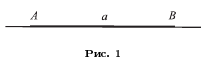
\includegraphics{mppics/ris-1}
\caption{}\label{1938/ris-1}
\bigskip
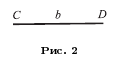
\includegraphics{mppics/ris-2}
\caption{}\label{1938/ris-2}
\bigskip
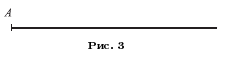
\includegraphics{mppics/ris-3}
\caption{}\label{1938/ris-3}
\end{wrapfigure}

Прямую обозначают обыкновенно двумя большими буквами, поставленными у двух каких-либо её точек.
Так, говорят:
«прямая $AB$» или «$BA$» (рис.~\ref{1938/ris-1}).

Часть прямой, ограниченная с обеих сторон, называется \rindex{отрезок}\textbf{отрезком};
отрезок обыкновенно обозначается двумя буквами, поставленными у его концов (отрезок $CD$, рис.~\ref{1938/ris-2}).
Иногда прямую или отрезок обозначают и одной буквой (малой);
например, говорят: «прямая $a$, отрезок $b$».

Иногда рассматривают прямую, ограниченную только с одной стороны, например в точке $E$ (рис.~\ref{1938/ris-3}).
О~такой прямой говорят, что она исходит из точки $E$;
её называют \rindex{луч}\textbf{лучом} или \rindex{полупрямая}\textbf{полупрямой}. 

\paragraph{Равенство и неравенство отрезков.}\label{1938/6}
\emph{Два отрезка равны, если они могут быть наложены один на другой так, что их концы совпадут.}
Положим, например, что мы накладываем отрезок $AB$ на
отрезок $CD$ (рис.~\ref{1938/ris-4}) так, чтобы точка $A$ совпала с точкой $C$ и чтобы прямая $AB$ пошла по прямой $CD$, если при этом концы $B$ и $D$ совпадут, то отрезки $AB$ и $CD$ равны;
в противном случае отрезки будут не равны, причём меньшим считается тот, который составит часть другого.


\begin{figure}[h!]
\centering
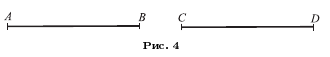
\includegraphics{mppics/ris-4}
\caption{}\label{1938/ris-4}
\end{figure}


Чтобы на какой-нибудь прямой отложить отрезок, равный данному отрезку, употребляют \textbf{циркуль} — прибор, известный учащимся из опыта.

\paragraph{Сумма отрезков.}\label{1938/7}
\rindex{сумма отрезков}
Суммой нескольких данных отрезков $AB$, $CD$, $EF,\dots$
(рис.~\ref{1938/ris-5}) называется такой отрезок, который получится следующим образом.
На какой-нибудь прямой берём произвольную точку $M$ и откладываем от неё отрезок $MN$, равный $AB$, затем от точки $N$ в том же направлении откладываем отрезок $NP$, равный $CD$, и отрезок $PQ$, равный $EF$.
Тогда отрезок $MQ$ и будет суммой отрезков $AB$, $CD$ и $EF$ (которые по отношению к этой сумме называются слагаемыми).
Подобным образом можно получить сумму какого угодно числа отрезков.

\begin{figure}[h!]
\centering
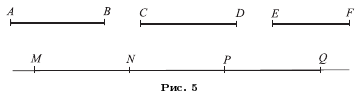
\includegraphics{mppics/ris-5}
\caption{}\label{1938/ris-5}
\end{figure}

Сумма отрезков обладает всеми свойствами суммы чисел;
так, она не зависит от порядка слагаемых (\so{переместительный закон}) и не изменяется, если некоторые слагаемые будут заменены их суммой (\so{сочетательный закон}).
Так:
\[AB+CD+EF=AB+EF+CD=EF+CD+AB=\dots\]
и
\[AB+CD+EF=AB+(CD+EF)=CD+(AB+EF)=\dots\]

\paragraph{Действия над отрезками.}\label{1938/8}
Из понятия о сумме выводятся понятия о разности отрезков, умножении и делении отрезков на число.
Так, разность отрезков $AB$ и $CD$ (если $AB>CD$) есть такой третий отрезок, сумма которого с $CD$ равна $AB$;
произведение отрезка $AB$ на число $3$ есть сумма трёх отрезков, из которых каждый равен $AB$;
частное от деления отрезка $AB$ на число $3$ есть третья часть $AB$ и так далее.

Если данные отрезки измерены какой-нибудь линейной единицей (например, сантиметром), и длины их выражены соответствующими числами, то длина суммы отрезков выразится суммой чисел, измеряющих эти отрезки, разность выразится разностью чисел и~т.~д.

\subsection*{Понятие об окружности}

\paragraph{Окружность.}\label{1938/9}
Если дадим циркулю произвольный раствор и, поставив одну его ножку остриём в какую-нибудь точку $O$ плоскости (рис.~\ref{1938/ris-6}), станем вращать циркуль вокруг этой точки, то другая его ножка, снабжённая карандашом или пером, прикасающимся к плоскости, опишет на плоскости непрерывную линию, все точки которой одинаково удалены от точки $O$.
Эта линия называется \rindex{окружность}\textbf{окружностью}, и точка $O$ — её \rindex{центр!окружности}\textbf{центром}.
Отрезки $OA$, $OB$, $OC,\dots$, соединяющие центр с какими-нибудь точками окружности, называются \rindex{радиус}\textbf{радиусами}.
Все радиусы одной окружности равны между собой.

Окружности, описанные одинаковыми радиусами, равны, так как они при совмещении их центров совмещаются всеми своими точками.
Прямая ($MN$, рис.~\ref{1938/ris-6}), проходящая через какие-нибудь две точки окружности, называется \rindex{секущая}\textbf{секущей}.

Отрезок ($EF$), соединяющий две какие-нибудь точки окружности, называется \rindex{хорда}\textbf{хордой}.

\begin{wrapfigure}{o}{39 mm}
\centering
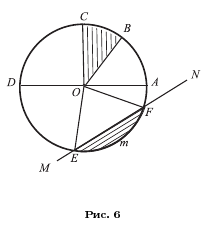
\includegraphics{mppics/ris-6}
\caption{}\label{1938/ris-6}
\bigskip
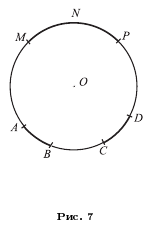
\includegraphics{mppics/ris-7}
\caption{}\label{1938/ris-7}
\end{wrapfigure}

Всякая хорда ($AD$), проходящая через центр, называется \rindex{диаметр}\textbf{диаметром}.
Диаметр равен сумме двух радиусов, и потому все диаметры одной окружности равны между собой.
Какая-нибудь часть окружности (например, $EmF$) называется \rindex{дуга}\textbf{дугой}.

О хорде ($EF$), соединяющей концы какой-нибудь дуги, говорят, что она \textbf{стягивает} эту дугу.

Дуга обозначается иногда знаком $\smallsmile$;
например, вместо «дуга $EmF$» пишут «${\smallsmile} EmF$».
Часть плоскости, ограниченная окружностью, называется \rindex{круг}\textbf{кругом}%
\footnote{Иногда слово «круг» употребляют в том же смысле, как и окружность.
Но этого следует избегать, так как употребление одного и того же термина для разных понятий может приводить к ошибкам.}%
.

Часть круга, заключённая между двумя радиусами (часть $COB$, покрытая штрихами на рис.~\ref{1938/ris-6}), называется \rindex{сектор}\textbf{сектором}, а часть, отсекаемая от круга какой-нибудь секущей (часть $EmF$), называется \rindex{сегмент}\textbf{сегментом}.



\paragraph{Равенство и неравенство дуг.}\label{1938/10}
Две дуги одной и той же окружности (или равных окружностей) равны между собой, если они могут быть совмещены так, что их концы совпадут.
Положим, например, что мы накладываем дугу $AB$ (рис.~\ref{1938/ris-7}) на дугу $CD$ так, чтобы точка $A$ совпала с точкой $C$ и дуга $AB$ пошла по дуге $CD$;
если при этом концы $B$ и $D$ совпадут, то совпадут и все промежуточные точки этих дуг, так как они находятся на одинаковом расстоянии от центра, значит, ${\smallsmile} AB={\smallsmile} CD$;
если же $B$ и $D$ не совпадут, то дуги не равны, причём та считается меньше, которая составит часть другой.

\paragraph{Сумма дуг.}\label{1938/11}
\rindex{сумма дуг}
Суммой нескольких данных дуг одинакового радиуса называется такая дуга того же радиуса, которая составлена из частей, соответственно равных данным дугам.
Так, если от произвольной точки $M$ (рис.~\ref{1938/ris-7}) окружности отложим часть $MN$, равную $AB$, и затем от точки $N$ в том же направлении отложим часть $NP$, равную $CD$, то дуга $MP$ будет суммой дуг $AB$ и $CD$.
Подобно этому можно составить сумму трёх и более дуг.

При сложении дуг одинакового радиуса их сумма может не уместиться на одной окружности, одна из дуг может частично покрыть другую.
В таком случае суммой дуг будет являться дуга, б\'{о}льшая целой окружности.
Так, например, при сложении дуги $AmB$ с дугой $CnD$ (рис.~\ref{1938/ris-8}) получаем дугу, состоящую из целой окружности и дуги $AD$.

\begin{figure}[h!]
\centering
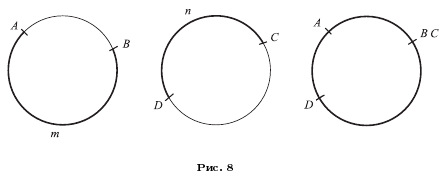
\includegraphics{mppics/ris-8}
\caption{}\label{1938/ris-8}
\end{figure}


Сумма дуг, как и сумма отрезков, обладает свойствами \textbf{переместительным} и \textbf{сочетательным}.

Из понятия о сумме дуг выводятся понятия о разности дуг, умножении и делении дуги на число, так же как и для отрезков.


\paragraph{Разделение геометрии.}\label{1938/12}
Геометрия разделяется на две части:
\textbf{планиметрию} и \textbf{стереометрию}.
Первая рассматривает свойства таких фигур, все части которых помещаются на одной плоскости;
вторая — свойства таких фигур, у которых не все части помещаются на одной плоскости.
